\documentclass[10pt, twoside]{article}
\usepackage{fancyhdr}
\usepackage{amsmath, amsthm, amssymb}
\usepackage[catalan]{babel}
\usepackage[titles]{tocloft}
\usepackage[utf8]{inputenc}
\usepackage[left=2.15cm, right=2.15cm, top=30mm, bottom=20mm]{geometry}
\usepackage{parskip}
\setlength{\parindent}{0pt} % Elimina la sangría de la primera línea de cada párrafo
\usepackage{titlesec}
\usepackage{hyperref}
\usepackage{float}
\usepackage{caption}
\usepackage{graphicx} % Required for inserting images
\usepackage[T1]{fontenc}
\usepackage{hyperref}
\usepackage{multirow}
\usepackage{subcaption}
\usepackage{booktabs}
\usepackage{bookmark}
\usepackage{graphicx}
\usepackage{setspace}
\usepackage{physics}
\usepackage{tikz}
\usepackage{tikz-3dplot}
\usepackage[outline]{contour} % glow around text
\usepackage{xcolor}
\usepackage{makeidx}
\usepackage{pgfplots}
\pgfplotsset{compat=1.18}
\usepackage{caption}
\setlength{\parskip}{11pt}
\usepackage{listings}

\captionsetup{labelfont=bf}

\begin{document}

\begin{titlepage}
\centering
{\Large Fonaments d'Enginyeria Química \\ MO70399 \par}
\vspace{2cm}
{\Huge \textbf{Pràctica 1:} \par}
\vspace{1cm}
{\Huge \textbf{Balanç de matèria} \par}
\vspace{1cm}
{\Large Grup B \par}
\vspace{0.5cm}
{\Large Torn 2 \par}
\vspace{0.5cm}
{\normalsize Baldi Garcia, Isaac: 1667260 \\ Barbens Calzadilla, Carla: 1666167 \\ Belmonte Leiva, Marc: 1619451 \\ Bujones Umbert, Jun Shan: 1549086 \\ Franco Avilés, Eric: 1666739 \\ Gómez Rubio, Miquel: 1668850 \\ González Barea, Eric: 1672980 \\ Jacas García, Eira: 1666616 \\ I NOMBRE DE PÀGINES AAAAAA\par}
\vspace{1cm}
{\Large Gener 2025 \par}
\vspace{2cm}

\includegraphics[width=0.4\textwidth]{Logo_UAB.png}

\end{titlepage}

\pagenumbering{gobble}
\renewcommand{\cftsecfont}{}
\renewcommand{\cftsecpagefont}{}
\renewcommand{\cftsecleader}{\cftdotfill{\cftdotsep}}
\renewcommand{\cftdotsep}{0.2}
\setlength{\cftbeforesecskip}{0.5em}
\setlength{\cftbeforesubsecskip}{0.5em}
\tableofcontents

\newpage
\pagenumbering{arabic}
\setcounter{page}{1}

\pagestyle{fancy}
\lhead{\textbf{Pràctica 1: Balanç de matèria}}
\rhead{\textbf{Fonaments d'Enginyeria Química}}

\begin{abstract}
En aquesta pràctica, el nostre objectiu era aplicar el balanç de matèria a un reactor de tanc agitat per on circula aigua mantenint el volum constant. Primerament, hem hagut de construir dues rectes de calibratge per poder relacionar les mesures insturmentals amb les dades que ens interessàva estudiar. Segonament, hem muntat un sistema en què podiem mesurar la variació de la concentració de sal d'una dissolució aquosa en el reactor en operació en continu. Així hem pogut comparar els resultats teòrics amb els experimentals.
\end{abstract}

\section{Calibratge}
Per dur a terme l'experiment primer hem calibrat els instruments que ho necessitaven, en aquest cas, la bomba i el conductímetre. 

\subsection{Recta de calibratge: concentració sal - conductiivitat dissolució}
Per calibrar el conductímetre hem preparat 7 dissolucions de sal i aigua de l'aixeta de diferents concentracions conegudes equiespaiades entre 0 g/L i 42 g/l. Després hem mesurat la conductivitat de cada dissolució i hem construit la següent taula.

GRAFIC I TAULA

Usant el programari Excel\copyright  hem construit aquest gràfic i n'hem generat l'equació de la recta.
Aquesta recta ens servira per trobar els valors de la concentració de sal dins del tanc a partir de les dades conductiomètriques.

\subsection{Corba de calibratge: cabal volumètric - revolucions per minut bomba}
Per calibrar la bomaba hem mesurat els volums d'aigua durant un període de temps determinat, fixant en cada mesura els rpm de la bomba i hem construit la següent taula.

GRAFIC I TAULA

Usant el programari Excel\copyright hem construit aquest gràfic i n'hem generat l'equació de la recta.
Aquesta recta ens servira per trobar els valors del cabal d'entrada a partir dels rpm de la bomba.

\section{Resultats experimentals}

\subsection{Volum del tanc}
Hem mesurat el volum del tanc: $\fbox{V=4L}$

Massa sal perquè concentració dins tanc sigui 40g/L: \fbox{$m_{sal} = 160g$}

\subsection{Temps de residència}
Temps de residència cabal=270.16 mL/min calculat: \fbox{$\tau= 888.38s$}

Temps de residència cabal=491.42 mL/min calculat: \fbox{$\tau = 488.39s$}

Temps de residència obtingut experimentalment pel cabal=270.16 mL/min : \fbox{$\tau_{regressió}=783.00s$}

Temps de residència obtingut experimentalment pel cabal=491.42 mL/min : \fbox{$\tau_{regressió}=448.67s$}

Error relatiu de $\tau_{Q_L = 270.16 mL/min} = \fbox{11,86 \%}$

Error relatiu de $\tau_{Q_L = 491.42 mL/min} = \fbox{8,132 \%}$

\subsection{Concentració del cabal de sortida}

\begin{figure}[hbt!]
    \centering
    \begin{subfigure}{0.45\textwidth}
        \centering
        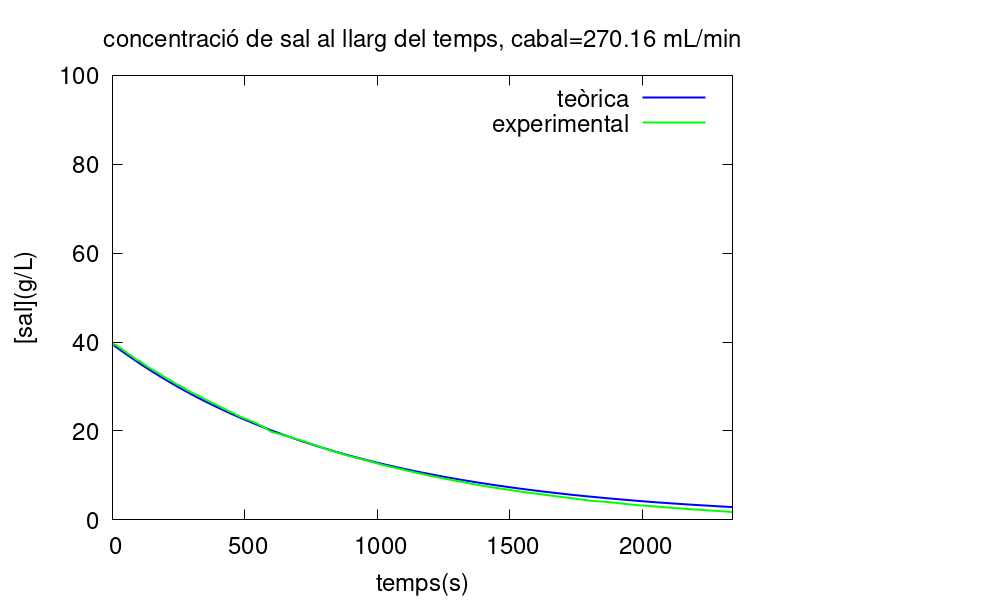
\includegraphics[width=\textwidth]{conc300.png}
        \caption{Concentració al llarg del temps per al cabal de 300 L/min (exp:270 L/min).}
        \label{fig:conc300}
    \end{subfigure}
    \hspace{0.025\textwidth}
    \begin{subfigure}{0.45\textwidth}
        \centering
        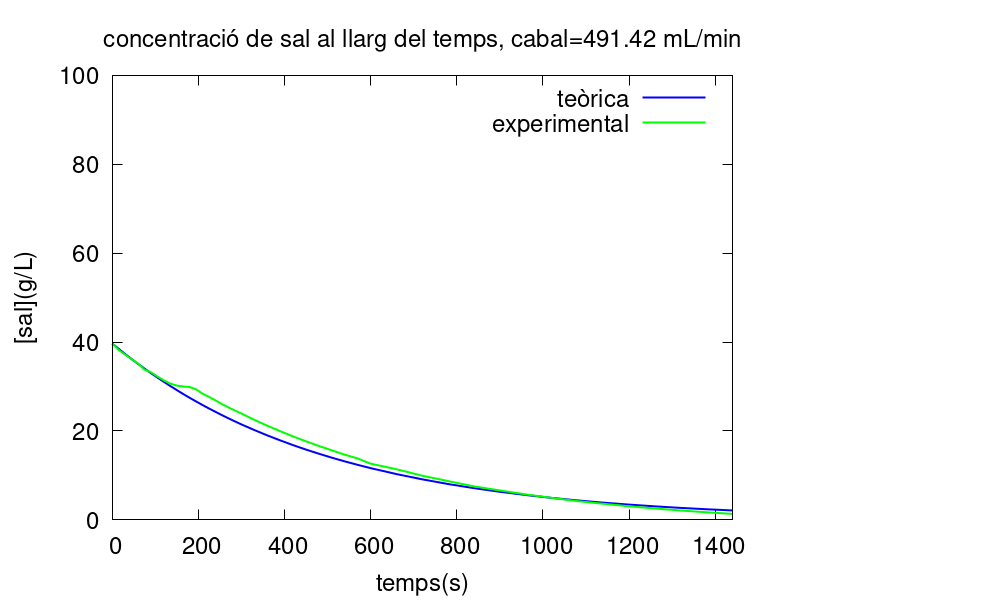
\includegraphics[width=\textwidth]{conc500.png}
        \caption{Concentració al llarg del temps per al cabal de 500 L/min (exp:491 L/min).}
        \label{fig:conc500}
    \end{subfigure}
    \caption{Concentració cabal de sortida}
    \label{fig:concs}
\end{figure}

Observem la figura \ref{fig:concs} a

\begin{figure}[hbt!]
    \centering
    \begin{subfigure}{0.45\textwidth}
        \centering
        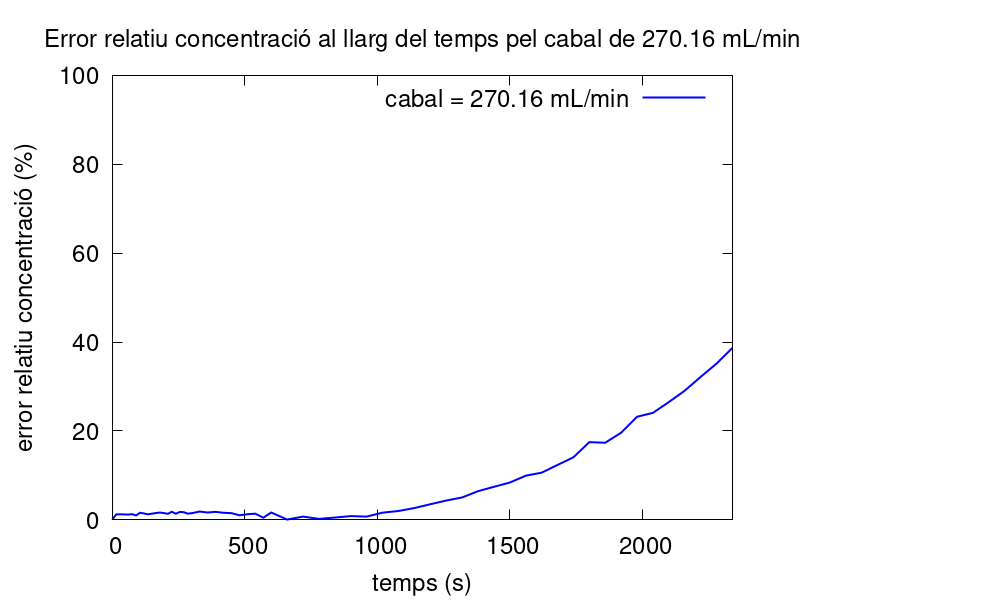
\includegraphics[width=\textwidth]{error300.png}
        \caption{Error relatiu per al cabal de 300 L/min (exp: 270.16 L/min).}
        \label{fig:error300}
    \end{subfigure}
    \hspace{0.025\textwidth}
    \begin{subfigure}{0.45\textwidth}
        \centering
        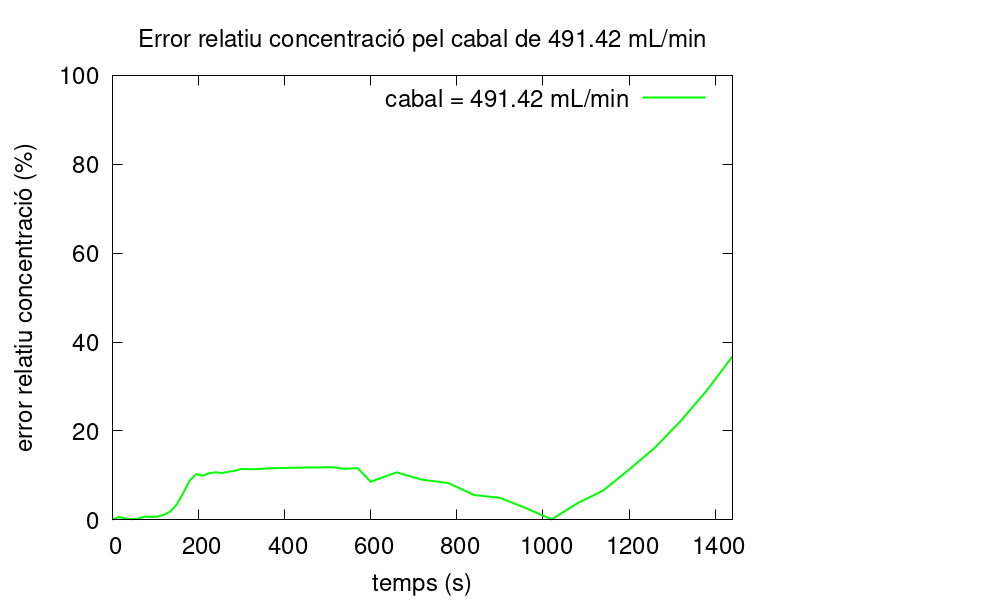
\includegraphics[width=\textwidth]{error500.png}
        \caption{Error relatiu per al cabal de 500 L/min (exp: 491.42 L/min).}
        \label{fig:error500}
    \end{subfigure}
    \caption{Error relatiu concentració cabal de sortida}
    \label{fig:errors}
\end{figure}

Observem la figura \ref{fig:errors} a

\section{Conclusions}

\section*{Annex}

\appendix

\section{Taules dades experimentals}

Taula conc sal - conductivitat

Taula cabal - rpm bomba

Taula conductivitat sal, concentracio sal, temps

\section{Hipòtesis i càlculs}

En aquesta pràctica hem considerat que el reactor de tanc agitat és ideal i, per tant, la mescla dins del tanc és perfecta. Això vol dir que podem assumir que la concentració de dins del tanc és la mateixa que la del cabal de sortida. Per aquesta raó, mesurem la conductiivitat de la dissolució quan encara està en el tanc.

També hem considerat que la concentració de sal de l'aigua de l'aixeta és tan petita que la podem despreciar. Per tant $c_{ref} = 0$.

Amb el volum del reactor ja podem calcular la quantitat de sal que necessitem perquè la concentració inicial dins del tanc sigui de $40g/L$. 
    $m_{sal} = V_{tanc}\frac{40g sal}{1L} = \fbox{160g sal}$
Amb el volum del tanc també podem calcular el temps de residència teòric per cada cabal.
    $\tau = V\frac{V}{Q_L}$

Calculem la concentració per a cada temps mitjançant l'equació proporcionada al guió:
\begin{equation}
    c(t) = c_{j_1} + (c_o-c_{j_1})\exp\left(-\frac{Q_L}{V}t\right) 
    \label{c(t)}   
\end{equation}

on $c_{j_1}$ és la concentració del cabal d'entrada. En aquest cas, és la concentració de sal que té la propia aigua d'aixeta (que hem considerat nul·la) i $c_o$ la concentració inicial de sal dins del tanc.
Grafic 1(teoric + exp cabal1), Gràfic2 (teo+exp cabal2)

Linealitzant l'equació \eqref{c(t)} fem el gràfic $\logc'(t)$ enfront $t$ i evaluant-ne el pendent obtenim el temps de residència. 
    \fbox{$\tau_{regressió} = resultat$}

Estudiem les diferències calculant l'error relatiu de les concentracions i del temps de residència, expressem el resultats en percentatges.

Error  relatiu  de  $c(t) = \frac{|c(t)_{teo} - c(t)_{exp} exp|}{c(t)_{teo}} 100$

Error relatiu de $\tau_{Q_L} = \frac{|\tau_{teo} - \tau_{exp}|}{\tau_{teo}} 100$

TAULA ERRORS RELATIUS CONCENTRACIó

A partir d'aquesta taula, hem construit el gràfic presentat a l'informe.

\end{document}